\documentclass[prb,aps,nobibnotes,twocolumn,doublespace,twocolumngrid,superbib]{revtex4}
%\documentclass[prb,aps,nobibnotes,superbib,preprint]{revtex4}

\usepackage{graphicx}
\usepackage{amsfonts}
\usepackage{amsmath}
\usepackage{bm}
\usepackage{alltt}
\usepackage{dcolumn} 
\usepackage{graphicx}
\makeatletter 
\makeatother

\begin{document}

\title{Linear scaling computation of the Fock matrix. VIII. Periodic \\
     boundaries, exact exchange and the Minimum Image Condition. }

\author{C. J. Tymczak}
\author{Valery Weber}
\author{Eric Schwegler}
\author{Matt Challacombe}

\affiliation{Theoretical Division, Los Alamos National Laboratory, Los Alamos,
New Mexico 87545 }

\affiliation{Larance Livermore}


\date{\today}
\begin{abstract}
A translationally invariant formulation of the Hartree-Fock $\Gamma$-point approximation
is achieved through introduction of the Minimum Image Convention.  This approximation is 
implemented  in the ONX algorithm [J.~Chem Phys, ], extending it to linear scaling 
computation of the periodic Hartree-Fock exchange matrix.  Convergence of the 
$\Gamma$-point approximation to the ${\bf k}$-space limit is demonstrated for 
magnesium oxide, ice and diamond.  True linear scaling is demonstrated for diamond and ice. 
\end{abstract}

\pacs{}

\maketitle

\footnotetext[1]{\tt tymczak@lanl.gov}
\footnotetext[2]{\tt vweber@lanl.gov}
\footnotetext[3]{\tt schwegler@llnl.gov}
\footnotetext[4]{\tt mchalla@lanl.gov}
\footnotetext[5]{\tt Preprint LA-UR 03-9043}

\section{INTRODUCTION}

Recent progress in linear scaling Density Functional Theory is enabling larger and 
more complex calculations of condensed phase systems.  In this approach, ${\cal O}(N)$
scaling with respect to system size, $N$, is achieved with algorithms that exploit 
quantum locality.  Applications of linear scaling algorithms to mineralogical problems 
\cite{MCraig04} and to energetic organic materials 
%\cite{} {\bf MORE HERE??} 
demonstrate the ability of these $N$-scaling algorithms to make valuable contributions well 
beyond the domain of conventional plane wave methods, which scale with the cube of system size.  

In the simulation of condensed phase systems, Gaussian basis functions have several 
advantages.  First, they are able to sustain all electron calculations into high 
pressure regimes where the effects of core electrons may be important. Second, they
support the application of Hartree-Fock and the hybrid Hartree-Fock/Density Functional 
Theory (HF/DFT) \cite{Gill92,Becke93,VBarone96,CAdamo99} through rapid, 
analytic evaluation of the exact Hartree-Fock exchange matrix.  
The Hartree-Fock approximation is often a fast, first approximation and also a starting point 
for correlated "wavefunction" methods.  The HF/DFT level of theory is also an important next 
in step in accuracy beyond the pure Generalized Gradient Approximation, which can often correctly 
describe  weak bonding \cite{}, deliver accurate band gaps \cite{} and treat the self-interaction 
energy of surfaces \cite{} {\bf( Should add to this list )}.  

To date, condensed phase HF and HF/DFT calculations have been carried out almost 
exclusively with the {\em ab initio} solid state program {\sc Crystal98} \cite{} (and
more recently {\sc Crystal03}), which employs conventional (non-direct) ${\cal O}(N^4)$ 
algorithms for evaluation of the HF exchange matrix.  The {\sc Crystal} programs employ the
formally (and numerically) correct ${\bf k}$-space integration algorithms that generate 
wavefunctions  inclusive of the necessary translational symmetries.   In the so-called 
$\Gamma$-pointapproximation,  these symmetries are omitted, but may be regained in the limit 
of a large super-cell,  or in the case of a disordered medium, simply a large cell.  With a more
tractable  formulation and asymptotic correctness in the limit of large systems, the
$\Gamma$-point  approximation represents an ideal basis for linear scaling exchange 
algorithms.   However, preliminary studies of the naive HF $\Gamma$-point were found (by us)
to converge to position dependent values different from the ${\bf k}$-space integration 
limit.   

In this paper we develop a translationally invariant definition of periodic Hartree-Fock exchange 
in the $\Gamma$-point limit.  This is accomplished through introducing a Minimum Image Convention
into the two-electron integral algorithm, similar to the approach employed in molecular 
dynamics when truncating short range potentials \cite{}.  We then go on to describe a modified 
{\sc ONX} algorithm \cite{} that achieves true linear scaling with the MIC $\Gamma$-point 
approximation, and numerical equivalence with the ${\bf k}$-space value in the limit of 
large super-cells.

%Many calculations of the electronic structure of condensed matter systems now make use
%of the exact exchange interaction 
%\cite{CPisani80,REvarestov83,MCausa88,JAlmlof94,RDovesi00}. 
%Whereas this has been a very
%important functional in the quantum chemistry community 
%\cite{PLowdin55,py,ASzabo89}, 
%until the advent of the hybrid functionals 
%\cite{Gill92,Becke93,ABecke96,Adamo99}, 
%this functional has had very little impact on the
%condensed matter electronic structure community. Now because of the accuracy obtainable with
%the hybrid functionals, it has become very desirable to include exact exchange into
%existing condensed matter electronic structure algorithms. 
%However, most of these calculations make use of ${\bf k}$-space integrations to 
%deal with the periodicity of the system \cite{RDovesi00}. However, this is not an ideal 
%situation 
%for linear scaling algorithms, where we would like to remove the need for doing
%${\bf k}$-space integrations altogether by increasing the system size. 
%However, when Gamma point only is attempted for exact exchange, a 
%significant problem arises. For the Gamma point, in the limit of large system size,
%we do not recover the ${\bf k}$-space energy per particle number; we do not have the correct
%limit as particle number increases.  
%
%In the proceeding sections we will first briefly review the Hartree
%Foch equations of motion. Next, we will illuminate the problem that exist
%for the calculation of the exchange matrix in the limit of the Gamma point for
%periodic systems. We then give a solution to this problem, and then we verify that
%the exchange matrix is correct in the limit of large systems as compared to a large 
%${\bf k}$-space calculation done with {\bf Crystal98}. 
%And finally, we verify that the exchange matrix build is indeed linear scaling
%for the dense diamond system.

%%%%%%%%%%%%%%%%%%%%%%%%%%%%%%%%%%%%%%%%%%%%%%%%%%%%%%%%%%%%%%%%%%%%%%%%%%%%%%%
%\newpage
%%%%%%%%%%%%%%%%%%%%%%%%%%%%%%%%%%%%%%%%%%%%%%%%%%%%%%%%%%%%%%%%%%%%%%%%%%%%%%%

\section{Periodic exact exchange}

In the conventional implementations of periodic boundary conditions, the 
Bloch functions 
\begin{equation}
\psi^{\bf k}_a({\bf r})  =  \sum_{\bf R} e^{i {\bf k}\cdot {\bf R}} \phi_a ({\bf r}-{\bf R}),
\label{Block}
\end{equation}
are often constructed from non-orthogonal functions local to the unit cell (UC). Here, the 
local function
$\phi_a$ is a Gaussian-Type Atomic Orbital (GTAO) centered on atom {\bf A}, while the 
sum on {\bf R} runs over the Bravais lattice defined by integer translates of the primitive 
lattice vectors {\bf a}, {\bf b} and {\bf  c}, and {\bf k} are the reciprocal 
Bravais Lattice vectors.

To date, rapid computation of the Hartree-Fock exchange interaction demands
the analytic evaluation of two-electron integrals, which is possible when the 
local basis functions are of Cartesian Gaussian type.  
Typically, these functions have the form
\begin{equation}
\phi_a ({\bf r}) = (x-A_x)^{l_a} (y-A_y)^{m_a} (z-A_z)^{n_a}{\large e}^{-\zeta_a ({\bf r}-{\bf A})^2}
\end{equation}
where the triad $\{l_a,m_a,n_a\}$ sets angular symmetry  
and the exponent $\zeta_a$ is chosen to describe a particular length scale. 
Gaussian basis functions are often contracted to approximate 
atomic eigenfunctions \cite{}.
 
With periodic boundary conditions, the exact Hartree-Fock exchange matrix in {\bf k}-space is 
\cite{MCausa88}
\begin{equation}
K_{ab} [{\bf k}] = \sum_{{\bf G}} K_{ab} [{\bf G}] e^{i {\bf k}\cdot {\bf G}}
\label{Kinkspace}
\end{equation}
where, 
\begin{equation}
K_{ab} [{\bf G}] = - \frac{1}{2}
\sum _{{\bf H N},c d} P_{cd}[{\bf N}]
\left(
      \phi        _a    
      \phi^{\bf H}_c    
{\big | }
      \phi^{\bf G}_b    
      \phi^{\bf H+N}_d  
\right) 
\label{CryEq}
\end{equation}
is defined in real space, and the two-electron integrals have been 
written in the notation:
\begin{eqnarray}
\left(
      \phi        _a  
      \phi^{\bf H}_c  
{\big | }
      \phi^{\bf G}_b  
      \phi^{\bf H+N}_d
\right)
= \quad\quad\quad\quad\quad 
 \quad\quad\quad\quad\quad  
 \quad\quad\quad\quad\quad 
\nonumber \\
\iint d {\bf r} d {\bf r}'
\frac{{\phi_a({\bf r}) \phi_c({\bf r}+{\bf H}})\phi_b({\bf r'}+{\bf G})\phi_d({\bf r'}+{\bf H}+{\bf{N})}}
{{\left|{\bf r}-{\bf r'}\right|}} 
\nonumber\\
\end{eqnarray}

The formally infinite sums over lattice vectors in Eq.~(\ref{CryEq}) involve 
many contributions that are in practice infinitesimal.  In part this is due to 
the decay between local basis function products $\phi_a \phi_c $; the product of
two Guassians centered at ${\bf A}$ and ${\bf C}$ decays also as a Gaussian with 
$|{\bf A}-{\bf C}|$. 
Truncation based purely on the overlap of Gaussian basis functions is reliable and
well controlled, leading efficiently to ${\cal O}(N)$ product terms.
Additionally, the density matrix is known to decay exponentially 
for non-metallic systems.  A radial cutoff $r_x$ defining the range of allowed exchange 
interactions may be used to exploit this fall off {\em a priori} by confining summation over 
${\bf N}$ \cite{REuwema74,CPisani80,RDovesi80,MCausa88} to only those terms that 
satisfy the imposed geometric constraints.  Radial cutoffs are also used to achieve
$N$-scaling of the exchange matrix in gas phase calculations by limiting the allowed range 
of atom centers ${\bf C}$ and ${\bf D}$ corresponding to matrix elements $P_{cd}$\cite{}.  

%%%%%%%%%%%%%%%%%%%%%%%%%%%%%%%%%%%%%%%%%%%%%%%%%%%%%%%%%%%%%%%%%%%%%%%%%%%%%%%
%\newpage
%%%%%%%%%%%%%%%%%%%%%%%%%%%%%%%%%%%%%%%%%%%%%%%%%%%%%%%%%%%%%%%%%%%%%%%%%%%%%%%

\section{Exchange at the $\Gamma$-point}\label{gammapoint}

The $\Gamma$-point approximation limits {\bf k}-space sampling to just the central cell, 
${\bf k} = 0$. With $N$-scaling algorithm, the effects of {\bf k}-space integration may be recouped 
with increasing cell-size. For the exact exchange matrix great care must be exercised in taking the limit
of decreasing {\bf k}-space. To this end, and to illustrate the problems asscoiated with this limit, let
us rewrite Eq.~(\ref{CryEq}) as 
\begin{equation}
K_{ab}[{\bf k}=0]=
\sum _{{\bf H G N} c d} P_{cd}[{\bf N}]
\left(
      \phi_a    
      \phi^{\bf H}_c    
{\big | }
      \phi^{\bf N}_b  
      \phi^{\bf N+G}_d  
\right)
\label{CryEq_1}
\end{equation}
However, we can not evalulate this expression because for the  $\Gamma$-point approximation 
$P_{cd}[{\bf N}]$ does not exist, we only have $P_{cd}[{\bf 0}]$. This leads us to two posibilities,
$P_{cd}[{\bf N}] = P_{cd}$ or $P_{cd}[{\bf N}] = P_{cd} \, \delta_{\bf N 0}$. But the first 
approximation leads to a divergent integral, so this is not correct. We are forced to consider the
second approximation, which  gives us the integral,
\begin{equation}
K_{ab}=
\sum _{{\bf H G} c d} P_{cd}[{\bf N}]
\left(
      \phi_a    
      \phi^{\bf H}_c    
{\big | }
      \phi_b  
      \phi^{\bf G}_d  
\right)
\label{CryEq_2}
\end{equation}
However, ther are two significant problems with this approximation. One, in this approximation the exact 
exchange potential, symmetric in the limit of infinite summation, has been asymmetrically truncated, 
resulting in a potential that depends on position  of the unit cell. 
And two, the $(a \rightarrow c, b \rightarrow d)$ permutational symmetry of the exchange 
integral is violated.  The translational non-invariance has a well understood analogue in classical
molecular dynamics, where the arbitrary truncation of short range potentials also leads to numerical 
artifacts in energies and forces.  In both cases, translational invariance is restored by 
introducing the Minimum Image Convention (MIC), which ensures that the distance between neighboring 
images is always used in computing interactions. In computation of the Hartree-Fock exchange matrix, 
the MIC $\Gamma$-point approximation is just
\begin{equation}
K_{ab}=
\sum _{{\bf H G} c d} P_{cd}
\left(
      \phi        _a    
      \phi^{\bf H}_c    
{\big | }
      \phi        _b    
      \phi^{\bf G}_d  
\right)_{\rm  MIC},
\label{MIC}
\end{equation}
where the MIC condition is applied in computation of the two electron integrals
at the contraction phase, ensuring that primitive charge distributions 
interact consistently over a minimum distance.  In particular, if the primitive basis 
function product $\phi_a \phi^{\bf H}_c$ is centered at ${\bf P}$ and the primitive product 
$\phi_b \phi^{\bf C}_d$ is at ${\bf Q}$, then the minimum image convention is 
applied to the interaction vector ${\bf PQ} \equiv {\bf P}-{\bf Q}$ using
\begin{subequations}
\begin{eqnarray}
{\bf pq}&=&{\bf M}^{-1} \cdot {\bf PQ} \\
pq_i & =& pq_i - {\tt ANINT} \left( pq_i \right) \\
{\bf PQ}_{\rm MIC}&=&{\bf M} \cdot {\bf pq} 
\end{eqnarray}
\end{subequations}
where ${\bf  M}$ is the $3 \times 3$ shape matrix of the unit cell, 
composed of the primative lattice vectors,
\begin{equation}
{\bf M} = \left( {\bf a}:{\bf b}:{\bf c} \right)
\end{equation}
This approach is completely general, and can be used at the primitive level with any modern approach
to computing two-electron integrals. Imposing this condition recovers translational invariace of the
exchange matrix, and in the limit of a sparce density matrix it also recovers the permutational
symmetry mentioned above.

Surprisingly, this work is the first to correctly define the exact Hartree-Fock 
exchange potential for periodic boundary conditions and the $\Gamma$-point approximation.  Moreover,
effects related to asymmetric truncation may also manifest in methods that perform incomplete 
${\bf k}$-space sampling, and may likewise benefit from employing the Minimum Image Convention. 

%%%%%%%%%%%%%%%%%%%%%%%%%%%%%%%%%%%%%%%%%%%%%%%%%%%%%%%%%%%%%%%%%%%%%%%%%%%%%%%
%\newpage
%%%%%%%%%%%%%%%%%%%%%%%%%%%%%%%%%%%%%%%%%%%%%%%%%%%%%%%%%%%%%%%%%%%%%%%%%%%%%%%

\section{Implementation}\label{implementation}

A general treatment of $\Gamma$-point Periodic Boundary Conditions has been implemented in the MondoSCF
suite of programs for linear scaling quantum chemistry.  A detailed account of these developments for 
pure Density Functional Theory has been given in a companion paper \cite{}, including the periodic 
development of the Quantum Chemical Tree Code ({\sc QCTC}) for performing $N$-scaling Coulomb summation.  

The Order N eXchange ({\sc ONX}) algorithm \cite{} for computing the gas phase exchange matrix 
has been modified by placing dual loops running over the lattice vectors 
${\bf H}$ and ${\bf G}$ around the original ONX loop structures.  Two ordered bra and ket distribution 
buffers are assembled for each lattice vector pair, which are then used to drive the original {\sc ONX}
 algorithm.
The Minimum Image Convention has been introduced into the primitive contraction stage, in the 
Vertical Recurrence Relations component of a symmetry driven Head-Gordon Pople \cite{} scheme for 
computing two-electron integrals.  While this implementation is linear scaling and simple, it suffers 
from a number of drawbacks that we will set forth in detail shortly, together with a more efficient 
algorithm able to achieve scalable parallelism \cite{}.

%%%%%%%%%%%%%%%%%%%%%%%%%%%%%%%%%%%%%%%%%%%%%%%%%%%%%%%%%%%%%%%%%%%%%%%%%%%%%%%
%\newpage
%%%%%%%%%%%%%%%%%%%%%%%%%%%%%%%%%%%%%%%%%%%%%%%%%%%%%%%%%%%%%%%%%%%%%%%%%%%%%%%

\section{Validation}

Periodic Hartree-Fock calculations were carried out using the periodic {\sc ONX} and {\sc QCTC}
programs from the {\sc MondoSCF} suite of linear scaling quantum chemistry programs.  The basic 
{\sc ONX} algorithm was described in \onlinecite{}, and its extension to periodic boundary conditions
outlined in Sections \ref{gammapoint} and \ref{implementation}.  The basic {\sc QCTC} method
was described in Ref.~\onlinecite{} and its extension to the condensed phase described in 
Ref.~\onlinecite{CTymczak03a}.   The linear scaling, Quartic Trace-ReSetting ({\sc TRS4}) density 
matrix solver has been used throughout, together with inverse congruence transformations provided
by sparse approximate {\sc AINV} \cite{}.  

Comparison is made to the Gaussian orbital periodic {\em ab initio} program {\sc Crystal98}, using
primarily basis sets designed for the condensed phase.  See Ref.~\onlinecite{TowlerLib} and references 
therein for details on these basis sets. 


Differences between the two programs are likely to arise from several factors.  First, {\sc Crystal98}
 uses an auxiliary fitting basis, while {\sc MondoSCF} does not.  Second, {\sc MondoSCF} uses several 
numerical thresholds, outlined in Appendix \ref{Thresholds}, in its linear scaling algorithms that can 
change the energy slightly.   In particular, a quadratic, variational dependence of the total energy
on the  matrix truncation threshold has recently been demonstrated for the {\sc TRS4} algorithm 
\cite{ANiklasson03}.  Finally, small super-cell calculations will typically be higher than the 
${\bf k}$-space integration limit.  

%%%%%%%%%%%%%%%%%%%%%%%%%%%%%%%%%%%%%%%%%%%%%%%%%%%%%%%%%%%%%%%%%%%%%%%%%%%%%%%
%\newpage
%%%%%%%%%%%%%%%%%%%%%%%%%%%%%%%%%%%%%%%%%%%%%%%%%%%%%%%%%%%%%%%%%%%%%%%%%%%%%%%

\begin{table}[h]
\caption{Progression of Hartree-Fock $\Gamma$-point super-cell calculations 
for MgO using the periodic RHF-MIC and RHF 8-511G/8-51G level of theory.  Comparison is 
made to a final value approaching the ${\bf k}$-space integration limit for the primitive cell.}
\label{MgOTable}
\center{\begin{tabular}{lrll}
\toprule
Program         & $N_{\rm at}$              & Energy (au)    & Energy/$N_{\rm at}$\\ 
\colrule
{\sc MondoSCF}       & 8$^g$    & -1098.4382     & -137.30478  \\
{\sc Crystal98}      & 16$^f$   & -2166.9440$^h$ & -135.43400$^h$ \\
{\sc MondoSCF}       & 16$^f$   & -2197.0564     & -137.31603  \\
{\sc Crystal98}      & 32$^g$   & -4394.5847     & -137.33077  \\
{\sc MondoSCF}       & 32$^g$   & -4394.4846     & -137.32764  \\
                     & 54$^f$   & -7415.8962     & -137.33141  \\
{\sc Crystal98}      & 64$^g$   & -8789.2484     & -137.33201  \\
{\sc MondoSCF}       & 64$^g$   & -8789.2494     & -137.33202  \\
                     & 128$^f$  & -17578.502     & -137.33205  \\
                     & 216$^g$  & -29663.729     & -137.33208  \\ 
\hline
{\sc Crystal98}$^i$  & 2$^f$    & -274.66415     & -137.33208  \\ 
\botrule 
\end{tabular}\\}
\raggedright{
{\hskip 0.330in}$^f$Triclinic \\
{\hskip 0.330in}$^g$Cubic \\
{\hskip 0.330in}$^h$Did not converge (See Ref.~\cite{BCivalleri02}) \\
{\hskip 0.330in}$^i 8\times8\times8$ ${\bf k}$-space integration grid  \\}
\end{table}

Table \ref{MgOTable} shows {\sc MondoSCF} $\Gamma$-point super-cell total energies for MgO 
at the RHF-MIC and RHF-C98 8-511G/8-51G level of theory.  See Ref.~\cite{TowlerLib} and 
references therein for details on these basis sets.  Comparison is made between RHF
$\Gamma$-point values obtained using the {\sc Cyrstal98} program, as well as with a final value 
approaching the ${\bf k}$-space integration limit for the primitive cell. 
Primitive cubic and triclinic cell coordinates for this system are listed in Appendix~\ref{Coordinates}.
The {\sc Crystal98} values were obtained as described in Ref.~\cite{BCivalleri02}, while the 
{\sc MondoSCF} values were obtained using the {\it tight} option, defining numerical thresholds 
delivering numbers precise to the digits quoted (8).  From these numbers, we see a fundamental 
difference between the RHF-MIC and RHF $\Gamma$-point values for small primitive cells; 
the periodic RHF-MIC approximation is convergent 

%%%%%%%%%%%%%%%%%%%%%%%%%%%%%%%%%%%%%%%%%%%%%%%%%%%%%%%%%%%%%%%%%%%%%%%%%%%%%%%
%\newpage
%%%%%%%%%%%%%%%%%%%%%%%%%%%%%%%%%%%%%%%%%%%%%%%%%%%%%%%%%%%%%%%%%%%%%%%%%%%%%%%

In Table~\ref{PIceTable}, total energies computed with the RHF-MIC $\Gamma$-point
super cell approach are listed for proton ordered ice \cite{}, using the 8-51G basis 
for Oxygen and the 5-11G$^*$ basis for Hydrogen.  A comparison is made to a final 
value obtained using {\sc Cyrstal98} with a $6\times6\times6$ ${\bf k}$-space integration grid
as explained in Ref.~\cite{PIceProceedure}.  The {\sc MondoSCF} values were obtained 
using the {\it tight} option, defining numerical thresholds that deliver total energies
precise to the digits quoted (8).  The primitive cubic cell coordinates used in these
ice calculations are listed in Appendix~\ref{Coordinates}.

\begin{table}[h]
\caption{Progression of $\Gamma$-point super-cell calculations of proton ordered ice
at the RHF-MIC/8-51G/5-11G$^*$ level of theory.   Comparison is made to a final value 
approaching the ${\bf k}$-space integration limit for the primitive cell.}
\label{PIceTable}
\center{\begin{tabular}{lrll}
\toprule
Program         & $N_{\rm H_20}$              & Energy (au)    & Energy/$N_{\rm H_2O}$\\ 
\colrule
{\sc MondoSCF}$^a$  & 2    &  -152.03025  &  -76.01512  \\
                    & 16   &  -1216.3003  &  -76.01877  \\
                    & 54   &  -4105.0163  &  -76.01882  \\
                    & 128  &  -9730.4090  &  -76.01882  \\
                    & 250  &  -19004.705  &  -76.01882  \\ 
\hline
{\sc Crystal98}$^b$  & 2   &  -152.03765  &  -76.01882  \\ 
\botrule
\end{tabular}\\}
\raggedright{
{\hskip 0.230in}$^a \Gamma$-point\\
{\hskip 0.230in}$^b 6\times6\times6$ ${\bf k}$-space integration grid \\}
\end{table}

%%%%%%%%%%%%%%%%%%%%%%%%%%%%%%%%%%%%%%%%%%%%%%%%%%%%%%%%%%%%%%%%%%%%%%%%%%%%%%%
%\newpage
%%%%%%%%%%%%%%%%%%%%%%%%%%%%%%%%%%%%%%%%%%%%%%%%%%%%%%%%%%%%%%%%%%%%%%%%%%%%%%%
\begin{table}[h]
\caption{Lattice Constants for the Diamond System for different 
system sizes, theory levels, and basis sets calculated at the $\Gamma$-point}
\label{DamondLC}
\center{\begin{tabular}{ccccc}
\toprule
$N_{\rm at}$  & Basis       &  HF     & PBE0 \\
\colrule
  64          & sto-3g      & ~3.587~ &  ~3.601    \\
  64          & 6-21g*      & ~3.575~ &  ~3.571    \\
\\
 216          & sto-3g      & ~3.500~ &  ~3.500    \\
 216          & 6-21g*      & ~3.500~ &  ~3.500    \\
\botrule
\end{tabular}\\}
\end{table}


Figure~\ref{DiamondLattice} compares the uniform diamond lattice potential computed 
by MondoSCF using the RHF-MIC $\Gamma$-point super-cell approximation to a {\sc Crystal98}
calculation using a two atom unit cell and a $12 \times 12 \times 12 ~{\bf k}$-space integration grid.
The {\sc MondoSCF} curves have been carried out with 64 atoms using {\it tight}
numerics, and with 512 atoms using a {\it loose} level of accuracy, but with the matrix
threshold further loosened to $\Huge \tau_{\rm \scriptscriptstyle MTRIX}=10^{-3}$. 
This modified level of approximation has been used to achieve the linear scaling shown 
in Fig.~\ref{DiamondScaling}. All calculations were carried out with a modified 6-31G basis set, 
with the most diffuse $sp$ exponent increased to 0.4, bringing the condition number 
of the overlap matrix into an acceptable range.  The computed lattice constants 
for diamond are $3.415$\AA~for the {\sc Crystal98} calculation, $3.421$\AA~for 
the 64 atom RHF-MIC calculation and $3.415$\AA~ for the 512 atom RHF-MIC calculation.
{\bf In comparison, the RHF/STO-3G lattice constant reported by Dovessi et.al \cite{RDovesi80b} 
is $3.59$\AA, while Euwema \cite{REuwema73} found a HF lattice constant of 3.54 using 13 
Gaussian basis functions per atom.  This should be compared to the experimental value of $3.57$\AA.
Thus, we are off by $0.15$\AA. }

\begin{figure}[h]
\caption{The uniform diamond lattice potential, computed by {\sc MondoSCF} using 
RHF-MIC with a slightly modified 6-31G basis.  The {\sc Crystal98} curve was computed
using a two atom unit cell and $12 \times 12 \times 12~{\bf k}$-space integration grid.}
\label{DiamondLattice}
{\center \includegraphics{Diamond_En_vs_a.ps} \par}
\end{figure}

%%%%%%%%%%%%%%%%%%%%%%%%%%%%%%%%%%%%%%%%%%%%%%%%%%%%%%%%%%%%%%%%%%%%%%%%%%%%%%%
%\newpage
%%%%%%%%%%%%%%%%%%%%%%%%%%%%%%%%%%%%%%%%%%%%%%%%%%%%%%%%%%%%%%%%%%%%%%%%%%%%%%%

\begin{figure}
\caption{The unrelaxed, uniaxial lattice potential of proton ordered ice \cite{}.
Comparison is made between a RHF-MIC/8-51G/5-11G$^*$ 250 molecule $\Gamma$-point super-cell 
calculation and a {\sc Crystal98} calculation carried out with a two molecule primitive
cell using a~$6\times6\times6$ ${\bf k}$-space integration grid.}
\label{IceEnergyVsLattice}
{\center \includegraphics{pIce_En_vs_a.ps}\par}
\end{figure}

Figure~\ref{IceEnergyVsLattice} shows the unrelaxed, uniaxial lattice potential of 
proton ordered ice \cite{} in the $a$ direction (see Appendix \ref{Coordinates} for the coordinate system).  
Comparison is made between a 250 molecule RHF-MIC $\Gamma$-point super-cell calculation performed 
with {\sc MondoSCF} and {\sc Crystal98} calculations carried out with a two molecule primitive
cell using a~$6\times6\times6$ ${\bf k}$-space integration grid, the 8-51G basis for Oxygen and the 
5-11G${^*}$ basis for Hydrogen.  The {\sc MondoSCF} {\it tight} option was used, delivering 
a relative accuracy of 8 digits. The potential minimum for the {\sc Crystal98} curve is $7.144$\AA~
and  for the {\sc MondoSCF} calculation $7.145$\AA.

%%%%%%%%%%%%%%%%%%%%%%%%%%%%%%%%%%%%%%%%%%%%%%%%%%%%%%%%%%%%%%%%%%%%%%%%%%%%%%%
%\newpage
%%%%%%%%%%%%%%%%%%%%%%%%%%%%%%%%%%%%%%%%%%%%%%%%%%%%%%%%%%%%%%%%%%%%%%%%%%%%%%%

\section{Scaling}

%%%%%%%%%%%%%%%%%%%%%%%%%%%%%%%%%%%%%%%%%%%%%%%%%%%%%%%%%%%%%%%%%%%%%%%%%%%%%%%
%\newpage
%%%%%%%%%%%%%%%%%%%%%%%%%%%%%%%%%%%%%%%%%%%%%%%%%%%%%%%%%%%%%%%%%%%%%%%%%%%%%%%

\begin{figure}[h]
\caption{CPU time for the exchange, Coulomb (scaled by 10)  and density 
matrix build (scaled by 20) of diamond using {\it loose} thresholding 
at the RHF-MIC/6-31G level of theory.}
\label{DiamondScaling}
{\centering \includegraphics{Timing_Diamond_ONX.ps} \par}
\end{figure}

In Fig.~\ref{DiamondScaling}, linear scaling is shown for diamond for 
building the exact exchange matrix, the Coulomb matrix, and solving for the density matrix. 
A modified 6-31G basis set was used, where the most diffuse $sp$ exponent was increased to 
0.4, bringing the condition number of the overlap matrix into an acceptable range.  A 
{\it loose} thresholding set (described in Appendix~\ref{Thresholds}) was used, with 
the matrix threshold further loosened to $\Huge \tau_{\rm \scriptscriptstyle MTRIX}=10^{-3}$.  
This was required to achieve a more aggressive truncation of the density matrix and an earlier 
onset of linear scaling for {\sc ONX}.  This level of approximation was used to generate 
the 512 atom lattice potential curve in Fig.~\ref{DiamondLattice}. While using tighter thresholds 
leads to more accurate results, it also postpones the onset of linear scaling. Because the 
calculations involving 800 atoms were just under the 4Gb available, it was important to 
demonstrate an early onset of linear scaling.  

%%%%%%%%%%%%%%%%%%%%%%%%%%%%%%%%%%%%%%%%%%%%%%%%%%%%%%%%%%%%%%%%%%%%%%%%%%%%%%%
%\newpage
%%%%%%%%%%%%%%%%%%%%%%%%%%%%%%%%%%%%%%%%%%%%%%%%%%%%%%%%%%%%%%%%%%%%%%%%%%%%%%%

\begin{figure}[h]
\caption{CPU time for the exchange, Coulomb and density 
matrix build (scaled by 10) of proton ordered ice using {\it tight}
thresholding at the RHF-MIC/8-51G/5-11G$^*$ level of theory.}
\label{IceScaling}
{\centering \includegraphics{Timing_pIce_ONX_1.ps} \par} 
\end{figure}

Figure~\ref{IceScaling} shows linear scaling for the exchange, Coulomb and density matrix
construction of proton ordered ice \cite{} using {\it tight} thresholds, the 8-51G basis set
for Oxygen and the 5-11G$^*$ basis set for Hydrogen.  An early onset of linear scaling 
is observed at about 50 water molecules, which is similar to the onset achieved in the gas 
phase \cite{ANiklasson03}.

%%%%%%%%%%%%%%%%%%%%%%%%%%%%%%%%%%%%%%%%%%%%%%%%%%%%%%%%%%%%%%%%%%%%%%%%%%%%%%%
%\newpage
%%%%%%%%%%%%%%%%%%%%%%%%%%%%%%%%%%%%%%%%%%%%%%%%%%%%%%%%%%%%%%%%%%%%%%%%%%%%%%%

\section{DISCUSSION}

A basic difference between the periodic {\sc MondoSCF} algorithms demonstrated 
here and other reduced scaling methods involving Gaussian basis functions is the 
ability to achieve true linear scaling for three-dimensional systems.  At the risk
of repetition; two-dimensions is trivial, three-dimensions is hard.  Another unique
feature of the linear scaling {\sc MondoSCF} algorithms is the use of continuous
thresholds that set cost to accuracy ratios on the fly.  Thus, as the gap closes and
a material heads toward a conducting state, periodic {\sc ONX} and {\sc TRS4} will
properly revert to ${\cal O}(N^2)$ and ${\cal O}(N^3)$ algorithms respectively.  This
should be compared with other approaches that use radial cutoffs to determine {\em a priori} 
the sparse matrix structure, range of exchange interactions, etc. 

Even for diamond, which is problematic due to its density, linear scaling was achieved.  
Albeit at the limit of utility, these {\it loose} $\Gamma$-point super-cell calculations were 
able to deliver lattice constants identical to those obtained with traditional 
${\bf k}$-space integration methods.  More efficient data structures for sparse 
matrix representation and a more efficient reformulation of {\sc ONX} will allow 
tighter calculations for difficult systems like diamond well beyond this mark, 
as will data parallelism.  

For less dense systems such as ice, the periodic {\sc MondoSCF} algorithms handily 
achieve an early onset of linear scaling using {\it tight} thresholding.  With parallelism,
this opens the prospect of performing hybrid HF/DFT simulations of fluids. 

Convergence of the MIC $\Gamma$-point super-cell calculations to values obtained with 
the well established {{\bf k}}-space integration methods in {\sc Crystal98} have been 
demonstrated to 8 digits.  We have not carried out calculations involving 
{\it d}-functions, because the use of fitting functions in {\sc Crystal98} makes
comparison to this level difficult.  We note important differences between the 
conventional truncation criteria employed in the {\sc Crystal98} $\Gamma$-point
approximation and the Hartree-Fock Minimum Image Condition developed in Section 
\ref{gammapoint}.  These differences diminish with increasing cell size and larger 
{\bf k}-space integration grids, following a surface to volume relationship 
as might be expected. {\bf OK HERE IS A HOLE IN OUR STORY.  OUR VALUES WITHOUT MIC
NEVER CONVERGED TO THE RIGHT NUMBER, BUT THE CRYSTAL VALUES DO?!!  WHY?  ARE WE
SURE THE NON-MIC VALUES REALLY CONVERGE TO THE WRONG NUMBER??}
Nevertheless, achieving high order translational invariance 
with the $\Gamma$-point approximation is likely to be important in {\em ab initio} 
molecular dynamics simulations employing the HF or HF/DFT model chemistries.

%%%%%%%%%%%%%%%%%%%%%%%%%%%%%%%%%%%%%%%%%%%%%%%%%%%%%%%%%%%%%%%%%%%%%%%%%%%%%%%
%\newpage
%%%%%%%%%%%%%%%%%%%%%%%%%%%%%%%%%%%%%%%%%%%%%%%%%%%%%%%%%%%%%%%%%%%%%%%%%%%%%%%

\section{CONCLUSIONS}

A new translationally invariant definition of the periodic Hartree-Fock 
$\Gamma$-point approximation has been introduced, based on inserting 
the Minimum Image Condition (MIC) into the contraction phase of periodically
summed two-electron integral algorithms.  This HF-MIC approach has been used 
to extend the {\sc ONX} algorithm for linear scaling computation of the exchange 
matrix to periodic boundary conditions.  Convergence of the HF-MIC $\Gamma$-point
super-cell approximation to the ${\bf k}$-space integration limit has been 
demonstrated for MgO and ice to better than 8 digits.  Differences between
the simply truncated $\Gamma$-point approximation implemented in the 
{\sc Crystal98} program and the HF-MIC were observed for small cells, but
largely disappear with increasing size. Linear scaling was demonstrated for
diamond and ice, including MIC-exchange, Coulomb and density matrix 
construction.   

We believe this work is the first proper definition of the $\Gamma$-point
Hartree-Fock potential, as well as the first demonstration of linear scaling
for periodic Hartree-Fock calculations.

%%%%%%%%%%%%%%%%%%%%%%%%%%%%%%%%%%%%%%%%%%%%%%%%%%%%%%%%%%%%%%%%%%%%%%%%%%%%%%%
%\newpage
%%%%%%%%%%%%%%%%%%%%%%%%%%%%%%%%%%%%%%%%%%%%%%%%%%%%%%%%%%%%%%%%%%%%%%%%%%%%%%%

\section*{ACKNOWLEDGMENTS}

We would like to acknowledge Tommy Sewell and Ed Kober for there advise
and support. We would also like to thank Anders Niklasson for his help
in preparation of this manuscript. 

%%%%%%%%%%%%%%%%%%%%%%%%%%%%%%%%%%%%%%%%%%%%%%%%%%%%%%%%%%%%%%%%%%%%%%%%%%%%%%%
%\newpage
%%%%%%%%%%%%%%%%%%%%%%%%%%%%%%%%%%%%%%%%%%%%%%%%%%%%%%%%%%%%%%%%%%%%%%%%%%%%%%%

\bibliographystyle{apsrmp} 
\bibliography{mondo_new} 

%%%%%%%%%%%%%%%%%%%%%%%%%%%%%%%%%%%%%%%%%%%%%%%%%%%%%%%%%%%%%%%%%%%%%%%%%%%%%%%
%\newpage
%%%%%%%%%%%%%%%%%%%%%%%%%%%%%%%%%%%%%%%%%%%%%%%%%%%%%%%%%%%%%%%%%%%%%%%%%%%%%%%

\appendix

\section{Coordinates of Validation Suite and Threshold Definitions}\label{Coordinates}
%
%
%
\begin{table}[p]
\caption{Fractional coordinates for the triclinic 2 atom unit cell of MgO, cooresponding to the 
         calculations reported in Table~\ref{MgOTable}.  Length of the unit cell is 
         $a=b=c=2.977776807$\AA, with angles $\alpha=\beta=\gamma=60^\circ$.}
\center{
\begin{tabular}{cccc}
\toprule
 Atom &  X  & Y  & Z \\
\colrule
Mg  &    0.000 &   0.000 &  0.000  \\
O   &    0.500 &   0.500 &  0.500  \\
\botrule
\end{tabular}}
\end{table}

\begin{table}[p]
\caption{Fractional coordinates for the cubic 8 atom unit cell of MgO, cooresponding to the 
         calculations reported in Table~\ref{MgOTable}.  Length of the unit cell is 
         $a=b=c=4.21121$\AA, with angles $\alpha=\beta=\gamma=90^\circ$.}
\center{
\begin{tabular}{cccc}
\toprule
 Atom &  X  & Y  & Z \\
\colrule
Mg &    0.000 &   0.000 &  0.000  \\
O  &    0.500 &   0.000 &  0.000  \\
Mg &    0.500 &   0.500 &  0.000  \\
O  &    0.000 &   0.500 &  0.000  \\
Mg &    0.500 &   0.000 &  0.500  \\
O  &    0.000 &   0.000 &  0.500  \\
Mg &    0.000 &   0.500 &  0.500  \\
O  &    0.500 &   0.500 &  0.500  \\
\botrule
\end{tabular}}
\end{table}


%
%
%
\begin{table}[p]
\caption{Fractional coordinates for the 8 atom unit cell of Diamond, cooresponding to the supercell 
calculations reported in Table~\ref{DiamondGammaPt}.  Dimensions of the cubic unit cell are 
$a=b=c=3.5700$\AA with angles  $\alpha=\beta=\gamma=90^\circ$.}
\center{
\begin{tabular}{cccc}
\toprule
 Atom &  X  & Y  & Z \\
\colrule
C &     0.125 &    0.125 &    0.125  \\
C &     0.375 &    0.375 &    0.375  \\
C &     0.625 &    0.625 &    0.125  \\
C &     0.875 &    0.875 &    0.375  \\
C &     0.625 &    0.125 &    0.625  \\
C &     0.875 &    0.375 &    0.875  \\
C &     0.125 &    0.625 &    0.625  \\
C &     0.375 &    0.875 &    0.875  \\
\botrule
\end{tabular}}
\end{table}
%
%
\begin{table}[p]
\caption{Fractional coordinates for the 2 molecule unit cell of proton ordered ice, cooresponding to 
the supercell calculations reported in Table~\ref{PIceTable}.  Dimensions of the cubic unit 
cell are $a=7.328$\AA, $b=7.920$\AA  and $c=4.400$\AA with angles  $\alpha=\beta=\gamma=90^\circ$. }
\center{
\begin{tabular}{cccc}
\toprule
 Atom &  X  & Y  & Z \\
\colrule
O &     0.063737 &  0.583443 &   0.000000 \\
H &     0.196106 &  0.583443 &   0.000000 \\
H &     0.018465 &  0.524173 &   0.177576 \\
O &     0.936263 &  0.916557 &   0.000000 \\
H &     0.980443 &  0.801105 &   0.000000 \\
H &     0.981535 &  0.975827 &   0.822424 \\
\botrule
\end{tabular}}
\end{table}

%%%%%%%%%%%%%%%%%%%%%%%%%%%%%%%%%%%%%%%%%%%%%%%%%%%%%%%%%%%%%%%%%%%%%%%%%%%%%%%
%\newpage
%%%%%%%%%%%%%%%%%%%%%%%%%%%%%%%%%%%%%%%%%%%%%%%%%%%%%%%%%%%%%%%%%%%%%%%%%%%%%%%

\section{Threshold Definitions}\label{Thresholds}

\begin{table}[p]
\caption{The various thresholds which enter into our three levels of accuracy}
\label{Table:AccurLevels}
\center{
\begin{tabular}{ccccc}
\toprule
Level  & Matrix & Penatration & QCTC/ONX & Distrabution \\ 
\colrule
loose     & $10^{-4}$ & $10^{-3}$ & $10^{-6}$ & $10^{-8}$ \\
good      & $10^{-5}$ & $10^{-5}$ & $10^{-8}$ & $10^{-10}$ \\
tight     & $10^{-6}$ & $10^{-7}$ & $10^{-10}$ & $10^{-12}$ \\
%verytight & $10^{-7}$ & $10^{-9}$ & $10^{-12}$ & $10^{-14}$ \\
\botrule
\end{tabular}}
\end{table}

%
%
%
%
%
%\begin{figure}
%\caption{Unit cell and its brava lattice vectors.}
%\label{figure:SimCell}
%{\centering \includegraphics{UnitCell_2.ps} \par}
%\end{figure}
%
%
%
%\begin{figure}
%\caption{For the Gamma point, the region in which atom $a$ has exchange interactions.}
%\label{figure:ExchangeRegion}
%{\centering \includegraphics{ExchangeRegion.ps} \par}
%\end{figure}
%
%
%
%\begin{figure}
%\caption{For ${{\bf k}}_{max}=\{1,1,1\}$, the region in which atom $a$ has exchange interactions.}
%\label{figure:ExchangeRegion_k111}
%{\centering \includegraphics{ExchangeRegion_k111.eps} \par}
%\end{figure}
%
%
%
%
%
%
%
%
%
%
\end{document}
